\documentclass{report}
\usepackage{graphicx, tikz-cd, float, titlepic, booktabs} % Required for inserting images
\usepackage{pgfplots}
\usepackage{multicol}
\usepackage{makecell}
\pgfplotsset{compat=1.15}
\usepackage{mathrsfs}
\usetikzlibrary{arrows}
\usepackage{amsmath, amssymb, amsthm, amsfonts, siunitx, physics, gensymb}
\AtBeginDocument{\RenewCommandCopy\qty\SI}
\usepackage[version=4]{mhchem}
\usepackage[most,many,breakable]{tcolorbox}
\usepackage{xcolor, fancyhdr, varwidth}
\usepackage[Glenn]{fncychap}
%Options: Sonny, Lenny, Glenn, Conny, Rejne, Bjarne, Bjornstrup
\usepackage{hyperref, cleveref}
\usepackage{icomma, enumitem} %comma as decimal and continue enumerate with [resume]
\usepackage{plimsoll} %use standard state symbol with \stst
\usepackage[danish]{babel}
\renewcommand{\cellalign}{cl}
\renewcommand{\theadalign}{cl}
\renewcommand\theadfont{\bfseries}
%%%%%%%%%%%%%%%%%%%%%%%%%%%%%%
% SELF MADE COLORS
%%%%%%%%%%%%%%%%%%%%%%%%%%%%%%
\definecolor{myg}{RGB}{56, 140, 70}
\definecolor{myb}{RGB}{45, 111, 177}
\definecolor{myr}{RGB}{199, 68, 64}
\definecolor{mytheorembg}{HTML}{F2F2F9}
\definecolor{mytheoremfr}{HTML}{00007B}
\definecolor{mylenmabg}{HTML}{FFFAF8}
\definecolor{mylenmafr}{HTML}{983b0f}
\definecolor{mypropbg}{HTML}{f2fbfc}
\definecolor{mypropfr}{HTML}{191971}
\definecolor{myexamplebg}{HTML}{F2FBF8}
\definecolor{myexamplefr}{HTML}{88D6D1}
\definecolor{myexampleti}{HTML}{2A7F7F}
\definecolor{mydefinitbg}{HTML}{E5E5FF}
\definecolor{mydefinitfr}{HTML}{3F3FA3}
\definecolor{notesgreen}{RGB}{0,162,0}
\definecolor{myp}{RGB}{197, 92, 212}
\definecolor{mygr}{HTML}{2C3338}
\definecolor{myred}{RGB}{127,0,0}
\definecolor{myyellow}{RGB}{169,121,69}
\definecolor{myexercisebg}{HTML}{F2FBF8}
\definecolor{myexercisefg}{HTML}{88D6D1}
%%%%%%%%%%%%%%%%%%%%%%%%%%%%%%%%%%%%%%%%%%%%%%%%%%%%%%%%%%%%%%%%%%%%%%
% Box environments for theorems and problems
%%%%%%%%%%%%%%%%%%%%%%%%%%%%%%%%%%%%%%%%%%%%%%%%%%%%%%%%%%%%%%%%%%%%%
\setlength{\parindent}{1cm}
%================================
% Question BOX
%================================
\makeatletter
\newtcbtheorem{question}{Opgave}{enhanced,
	breakable,
	colback=white,
	colframe=myb!80!black,
	attach boxed title to top left={yshift*=-\tcboxedtitleheight},
	fonttitle=\bfseries,
	title={#2},
	boxed title size=title,
	boxed title style={%
			sharp corners,
			rounded corners=northwest,
			colback=tcbcolframe,
			boxrule=0pt,
		},
	underlay boxed title={%
			\path[fill=tcbcolframe] (title.south west)--(title.south east)
			to[out=0, in=180] ([xshift=5mm]title.east)--
			(title.center-|frame.east)
			[rounded corners=\kvtcb@arc] |-
			(frame.north) -| cycle;
		},
	#1
}{def}
\makeatother
%================================
% DEFINITION BOX
%================================

\newtcbtheorem[number within=section]{definition}{Definition}{enhanced,
	before skip=2mm,after skip=2mm, colback=red!5,colframe=red!80!black,boxrule=0.5mm,
	attach boxed title to top left={xshift=1cm,yshift*=1mm-\tcboxedtitleheight}, varwidth boxed title*=-3cm,
	boxed title style={frame code={
					\path[fill=tcbcolback]
					([yshift=-1mm,xshift=-1mm]frame.north west)
					arc[start angle=0,end angle=180,radius=1mm]
					([yshift=-1mm,xshift=1mm]frame.north east)
					arc[start angle=180,end angle=0,radius=1mm];
					\path[left color=tcbcolback!60!black,right color=tcbcolback!60!black,
						middle color=tcbcolback!80!black]
					([xshift=-2mm]frame.north west) -- ([xshift=2mm]frame.north east)
					[rounded corners=1mm]-- ([xshift=1mm,yshift=-1mm]frame.north east)
					-- (frame.south east) -- (frame.south west)
					-- ([xshift=-1mm,yshift=-1mm]frame.north west)
					[sharp corners]-- cycle;
				},interior engine=empty,
		},
	fonttitle=\bfseries,
	title={#2},#1}{def}

%================================
% NOTE BOX
%================================

\usetikzlibrary{arrows,calc,shadows.blur}
\tcbuselibrary{skins}
\newtcolorbox{note}[1][]{%
	enhanced jigsaw,
	colback=gray!20!white,%
	colframe=gray!80!black,
	size=small,
	boxrule=1pt,
	title=\textbf{Note:},
	halign title=flush center,
	coltitle=black,
	breakable,
	drop shadow=black!50!white,
	attach boxed title to top left={xshift=1cm,yshift=-\tcboxedtitleheight/2,yshifttext=-\tcboxedtitleheight/2},
	minipage boxed title=1.5cm,
	boxed title style={%
			colback=white,
			size=fbox,
			boxrule=1pt,
			boxsep=2pt,
			underlay={%
					\coordinate (dotA) at ($(interior.west) + (-0.5pt,0)$);
					\coordinate (dotB) at ($(interior.east) + (0.5pt,0)$);
					\begin{scope}
						\clip (interior.north west) rectangle ([xshift=3ex]interior.east);
						\filldraw [white, blur shadow={shadow opacity=60, shadow yshift=-.75ex}, rounded corners=2pt] (interior.north west) rectangle (interior.south east);
					\end{scope}
					\begin{scope}[gray!80!black]
						\fill (dotA) circle (2pt);
						\fill (dotB) circle (2pt);
					\end{scope}
				},
		},
	#1,
}
%================================
% EXAMPLE BOX
%================================
\newtcbtheorem[number within=section, use counter from=definition]{Example}{Example}
{%
	colback = myexamplebg
	,breakable
	,colframe = myexamplefr
	,coltitle = myexampleti
	,boxrule = 1pt
	,sharp corners
	,detach title
	,before upper=\tcbtitle\par\smallskip
	,fonttitle = \bfseries
	,description font = \mdseries
	,separator sign none
	,description delimiters parenthesis
}
{ex}
%================================
% THEOREM BOX
%================================

\tcbuselibrary{theorems,skins,hooks}
\newtcbtheorem[number within=section, use counter from=definition]{Theorem}{Theorem}
{%
	enhanced,
	breakable,
	colback = mytheorembg,
	frame hidden,
	boxrule = 0sp,
	borderline west = {2pt}{0pt}{mytheoremfr},
	sharp corners,
	detach title,
	before upper = \tcbtitle\par\smallskip,
	coltitle = mytheoremfr,
	fonttitle = \bfseries\sffamily,
	description font = \mdseries,
	separator sign none,
	segmentation style={solid, mytheoremfr},
}
{th}

%%%%%%%%%%%%%%%%%%%%%%%%%%%%%%%%%%%%%%%%%%%%%%%%%%%%%%%%%%%%%%%%%
% SELF MADE COMMANDS
%%%%%%%%%%%%%%%%%%%%%%%%%%%%%%
\newcommand{\sol}{\setlength{\parindent}{0cm}\textbf{\textit{Løsning:}}\setlength{\parindent}{1cm}}
%%%%%%%%%%%%%%%%%%%%%%%%%%%%%%%%%
\usepackage[tmargin=2cm,rmargin=1in,lmargin=1in,margin=0.85in,bmargin=2cm,footskip=.2in]{geometry}\pagestyle{fancy}
\lhead{Terminsprøve}

\title{Terminsprøve\\
{\Large \textbf{Kemi A}}}
\date{\today}

\begin{document}
\maketitle
\begin{note}
  Databog fysik kemi (2007) er benyttet ved beregningerne.
\end{note}
\section*{Opgave 1: PEF - en ny type bioplast}
\sol \\
\textbf{a.}
En strukturisomer til A, som indeholder en aldehydgruppe ses i \cref{fig:isomer}.
\begin{figure}[H]
\begin{center}
  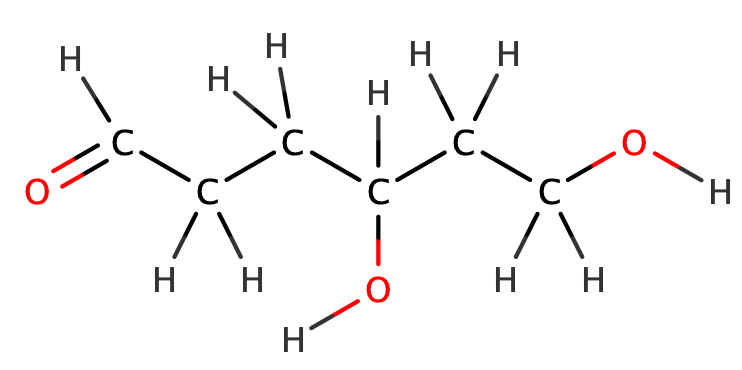
\includegraphics[width=\textwidth]{isomer.png}
\end{center}
\caption{Strukturisomer til stof A}
\label{fig:isomer}
\end{figure}
\noindent \textbf{b.}
For at bestemme strukturen for B, finder vi først den empiriske formel.
Fra elementaranalysen har vi, at der i 100 g af stoffet må være
\begin{equation*}
\begin{split}
  n(\ce{C} )&=\frac{38,70 \;\unit{g} }{12,01 \;\unit{g/mol} }= 3,222 \;\unit{mol} \\
  n(\ce{H} )&=\frac{9,74 \;\unit{g} }{1,008 \;\unit{g/mol} }= 9,663 \;\unit{mol} \\
  n(\ce{O})&=\frac{51,55 \;\unit{g} }{16,00 \;\unit{g/mol} }= 3,222 \;\unit{mol} 
\end{split}
\end{equation*}
Vi beregner nu stofmængdeforholdene.
\begin{equation*}
\begin{split}
  \frac{n(\ce{C} )}{n(\ce{O} )}&=\frac{3,222 \;\unit{mol} }{3,222 \;\unit{mol} }= 1\\
  \frac{n(\ce{H} )}{n(\ce{O} )}&=\frac{9,663 \;\unit{mol} }{3,222 \;\unit{mol} }=2,999 \approx 3
\end{split}
\end{equation*}
Forholdet mellem stofmængderne af C, H og O er altså med stor nøjagtighed 1:3:1.
Stoffet B's empiriske formel må da være \ce{CH3O}.

Da det oplyses, at B indeholder netop to \ce{O}-atomer, så må molekylformlen for B være \ce{C2H6O2}.
Siden B er en alkohol og har en symmetrisk struktur, så må den eneste mulige struktur for B være som i \cref{fig:B}.
\begin{figure}[H]
\begin{center}
  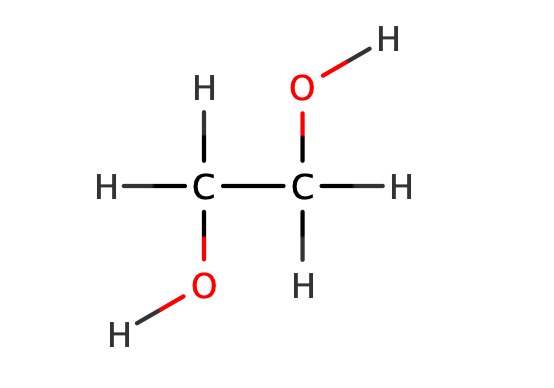
\includegraphics[width=0.5\textwidth]{B.png}
\end{center}
\caption{Struktur for B}
\label{fig:B}
\end{figure}
\noindent \textbf{c.}
Vi ser på \cref{fig:CDE}, at C indeholder både en hydroxy-gruppe og en aldehyd-gruppe, hvor D indeholder to aldehydgrupper, og E indeholder to syre-grupper.
\begin{figure}[H]
\begin{center}
  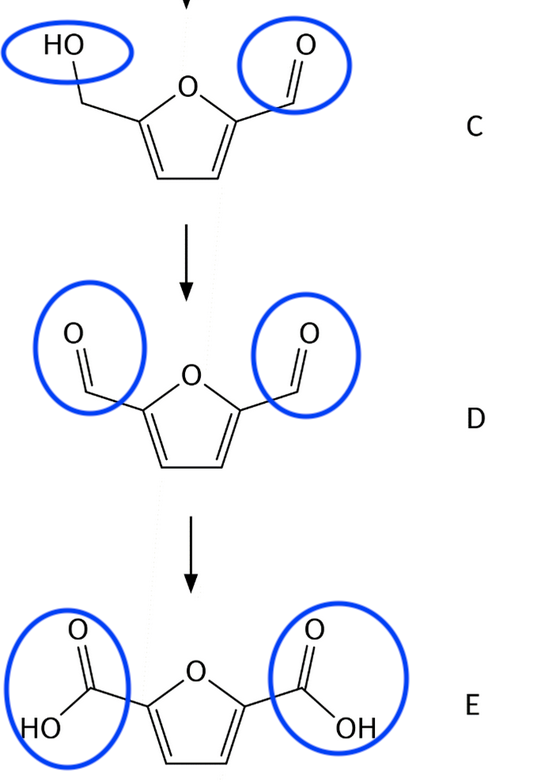
\includegraphics[width=0.5\textwidth]{CDE.png}
\end{center}
\caption{Strukturer for C, D og E med vigtige grupper markeret}
\label{fig:CDE}
\end{figure}
Stof E er det eneste stof, der er en carboxylsyre, og dets IR-spektrum må da indeholde et meget bredt bånd ved omkring 2500-3500 \;\unit{cm ^{-1}}, der er grundet \ce{O-H}-strækningsvibrationerne i carboxylsyre-gruppen.
Vi ser, at det første IR-spektrum må passe til stof E (\cref{fig:IRE}).
\begin{figure}[H]
\begin{center}
  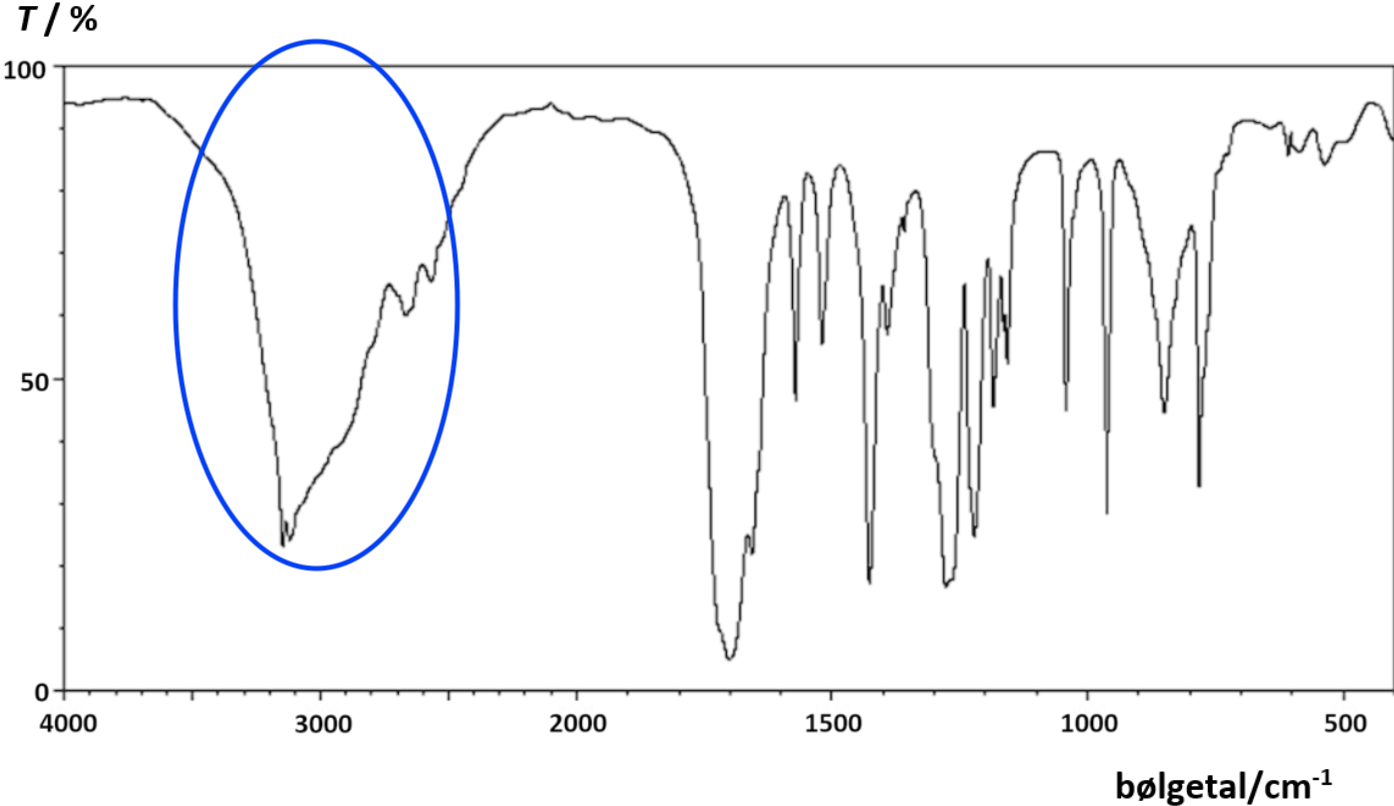
\includegraphics[width=0.7\textwidth]{IRE.png}
\end{center}
\caption{IR-spektrum for stof E}
\label{fig:IRE}
\end{figure}
Tilsvarende er stof C det eneste stof, der indeholder en hydroxy-gruppe, og dets IR-spektrum må da indeholde et bredt bånd ved omkring 3100-3600 \;\unit{cm ^{-1}}, der er grundet \ce{O-H}-strækningsvibrationerne i hydroxy-gruppen.
Vi ser, at det sidste IR-spektrum må passe til stof C (\cref{fig:IRC}).
\begin{figure}[H]
\begin{center}
  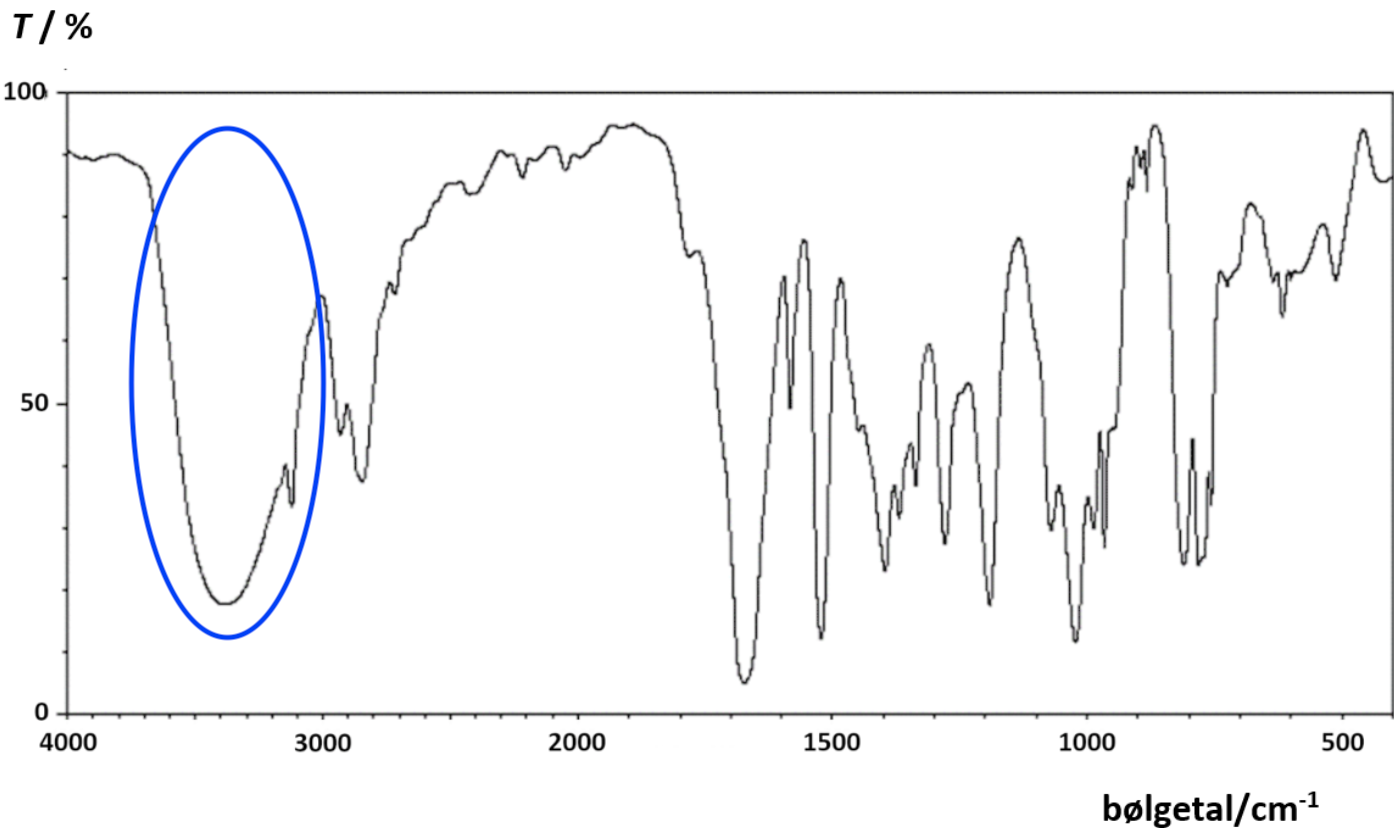
\includegraphics[width=0.7\textwidth]{IRC.png}
\end{center}
\caption{IR-spektrum for C}
\label{fig:IRC}
\end{figure}
\section*{Opgave 2: 1080 - et rodenticid}
\sol \\
\textbf{a.}
Reaktionen er en substitutionsreaktion, da der er tale om et atom, der udskiftes med et andet atom (eller her en ion).
Det understøttes af reaktionsskemaet, hvor vi ser chlorid blive udskiftet med fluorid.
Altså er reaktionen en substitutionsreaktion.\\[1ex]
\textbf{b.}
Siden $pK_s=2,59$, så er der tale om en middelstærk syre.
Der gælder da
\begin{equation*}
\begin{split}
K_s=\frac{\left[\ce{H3O+} \right]^2}{c_s-\left[\ce{H3O+} \right]} &\implies \left[\ce{H3O+} \right]=\frac{-K_s + \sqrt{K_s^2 - 4 \cdot \left(-K_s \cdot c_s\right) } }{2}\\
  &\iff pH=- \log\left(\frac{-10 ^{-pK_s} \;\unit{\textsc{m}} + \sqrt{\left(10 ^{-pK_s}\;\unit{\textsc{m}} \right)^2 - 4 \cdot \left(-10 ^{-pK_s} \;\unit{\textsc{m}} \cdot c_s\right) } }{2 \;\unit{\textsc{m}} }\right) 
\end{split}
\end{equation*}
fordi $pH=-\log\left(\frac{[\ce{H3O+} ]}{\unit{\textsc{m}}}\right) $.
Vi indsætter de kendte værdier og udregner pH.
\begin{equation*}
\begin{split}
  pH&=- \log\left(\frac{-10 ^{-pK_s} \;\unit{\textsc{m}}  + \sqrt{\left(10 ^{-pK_s} \;\unit{\textsc{m}} \right)^2 - 4 \cdot \left(-10 ^{-pK_s} \;\unit{\textsc{m}} \cdot c_s\right) } }{2 \;\unit{\textsc{m}} }\right) \\
  &=-\log\left(\frac{-10^{-2,59}\;\unit{\textsc{m}} + \sqrt{\left(10^{-2,59}\;\unit{\textsc{m}}\right)^2-4 \cdot \left(-10^{-2,59}\;\unit{\textsc{m}} \cdot 1,3 \cdot 10 ^{-4} \;\unit{\textsc{m}} \right) } }{2 \;\unit{\textsc{m}} }\right) \\
  &\approx 3,91
\end{split}
\end{equation*}
Altså vil det sige, at i opløsningen ved $25 \;\unit{\celsius} $ er $pH=3,91$. \\[1ex]
\textbf{c.}
Vi lader \ce{HFle} betegne fluorethansyre.
Så bliver titreringsreaktionen
\[
\ce{HFle(aq) + OH-(aq) -> Fle-(aq) + H2O(l)}
\] 
Vi ser, at reaktionsforholdet mellem fluorethansyre og \ce{NaOH} er 1:1.

Grundet indikatoren skifter blandingen farve ved ækvivalenspunktet, hvor $n(\ce{HFle} )=n(\ce{NaOH} )$.
Vi aflæser (se \cref{fig:tit}), at der ved ækvivalenspunktet er tilsat $13,3 \;\unit{mL} $ af \ce{NaOH}-opløsningen. 
\begin{figure}[H]
\begin{center}
  
\includegraphics[width=\textwidth]{tit.png}
\end{center}
\caption{Aflæsning af den tilsatte volumen \ce{NaOH}-opløsning ved ækvivalenspunktet}
\label{fig:tit}
\end{figure}
Ved ækvivalenspunktet gælder der 
\begin{equation*}
\begin{split}
  n(\ce{HFle} )=n(\ce{NaOH} ) &\iff c(\ce{HFle} ) \cdot V(\ce{HFle} ) = c(\ce{NaOH} ) \cdot V(\ce{NaOH} )\\
  &\iff c(\ce{HFle} )  = \frac{c(\ce{NaOH} ) \cdot V(\ce{NaOH} )}{V(\ce{HFle} )}
\end{split}
\end{equation*}
Vi indsætter nu de kendte værdier og udregner $c(\ce{HFle} )$.
\begin{equation*}
\begin{split}
  c(\ce{HFle} ) &= \frac{c(\ce{NaOH} ) \cdot V(\ce{NaOH} )}{V(\ce{HFle} )}\\
  &=\frac{0,089 \;\unit{\textsc{m}} \cdot 13,3 \;\unit{mL}  }{10,0 \;\unit{mL} }\\
  &\approx 0,118 \;\unit{\textsc{m}}  
\end{split}
\end{equation*}
Stofmængdekoncentrationen af fluorethansyre i den vandige opløsning er altså $c(\ce{HFle} )=0,118 \;\unit{\textsc{m}}  $.\\[1ex]
\textbf{d.}
Ved pH $=6,5$ aflæses (se \cref{fig:fordeling}) for coumatetralyl:
\begin{equation*}
\begin{split}
  \text{Blå kurve}: \quad x_B=0,88 \quad (88 \;\%)\\
\end{split}
\end{equation*}
Ved pH $=6,5$ er procentdelen af coumatetralyl, der findes på baseform altså $88 \;\%$.
\begin{figure}[H]
\begin{center}
  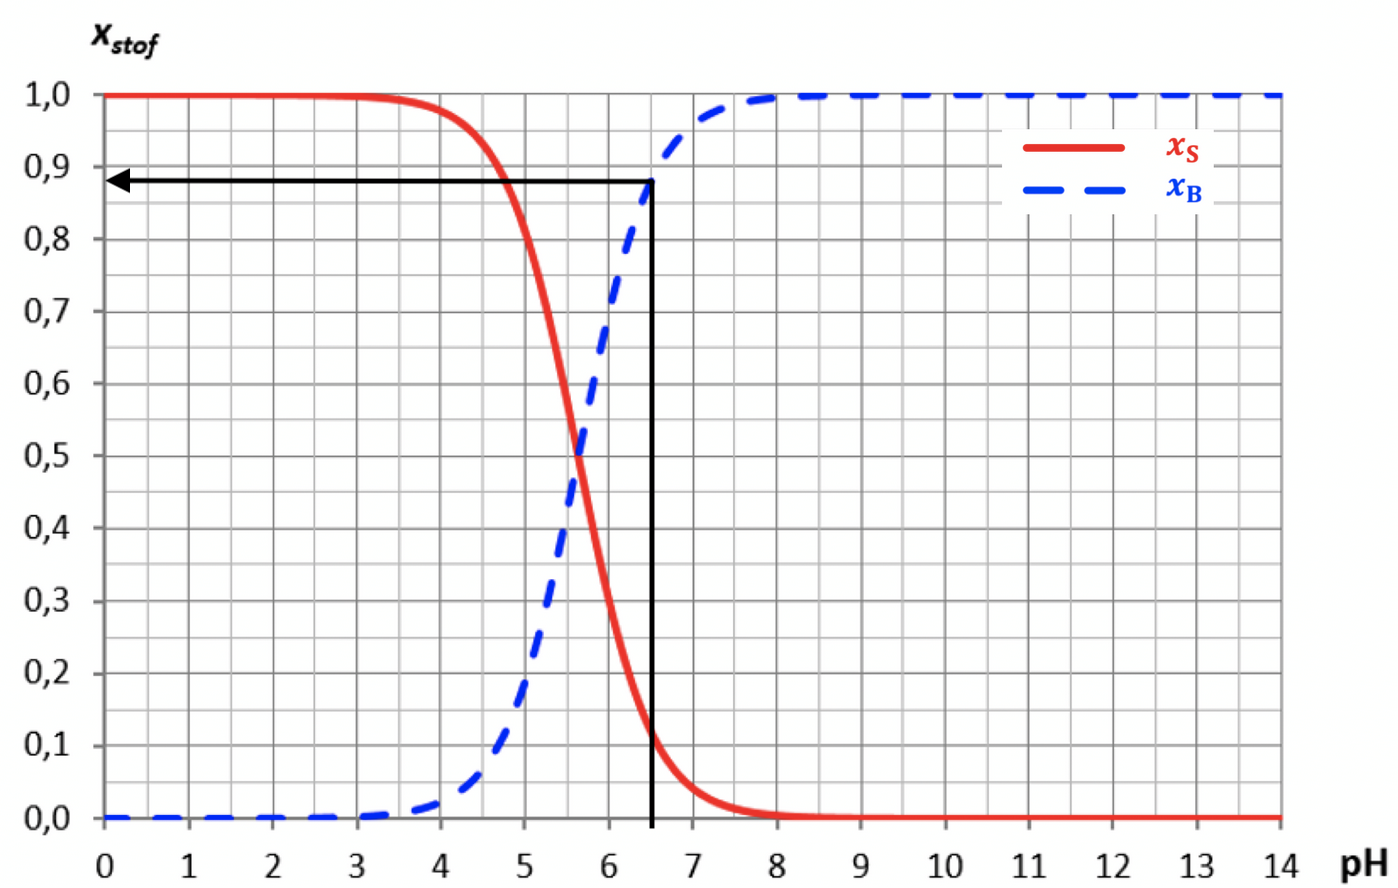
\includegraphics[width=0.7\textwidth]{fordeling.png}
\end{center}
\caption{Aflæsning på fordelingsdiagrammet}
\label{fig:fordeling}
\end{figure}
\noindent \textbf{e.}
I \cref{fig:SB} ses det, at at baseformen B i høj grad må have en stærk polær karakter, da det er en ion.
Tilsvarende er syreformen S overvejende upolær, da den indeholder virkeligt mange hydrofobe grupper (f.eks. \ce{C-H}).
Altså kan baseformen B let opløses i vand mens opløseligheden i octan-1-ol er lav.
Modsat kan syreformen S let opløses i octan-1-ol, mens opløseligheden i vand er lav.

Fra fordelingsdiagrammet \cref{fig:fordeling} ser vi, at når pH vokser, så aftager andelen af coumatetralyl på syreform, hvor andelen af coumatetralyl på baseform vokser.
Det er da klart, at så må andelen af coumatetralyl opløst i octan-1-ol aftager, og andelen af coumatetralyl opløst i vand vokser.

Når pH vokser må $D$ derfor aftage, hvilket vil sige, at $\log\left(D\right) $ også aftager. 
\begin{figure}[H]
\begin{center}
  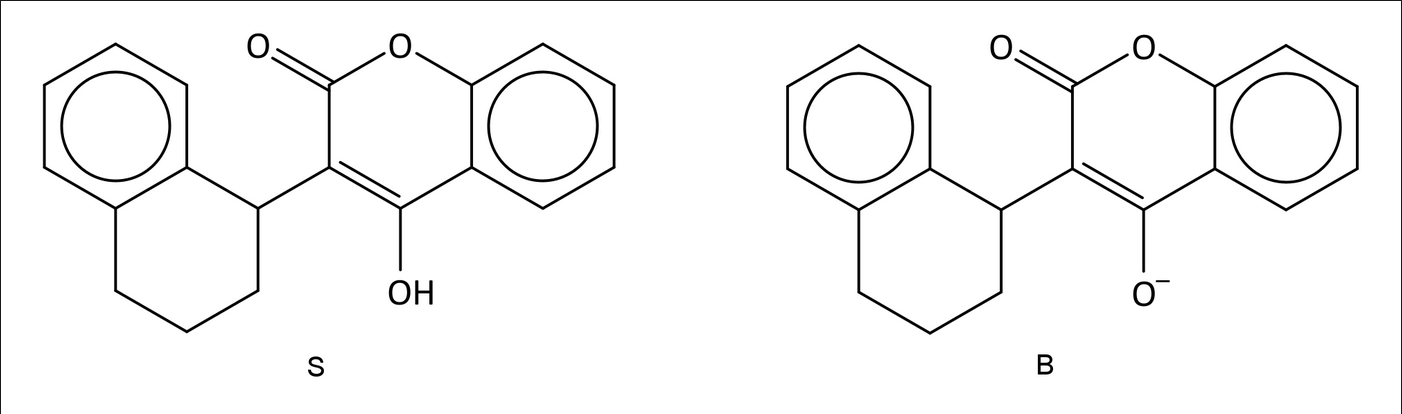
\includegraphics[width=0.7\textwidth]{SB.png}
\end{center}
\caption{Strukturer for coumatetralyl}
\label{fig:SB}
\end{figure}

\section*{Opgave 3: Mango}
\sol \\
\textbf{a.}
Den funktionelle gruppe med højsest prioritet er aldehyudgruppen.
Navnet får derfor suffikset -al og \ce{C}-atomerne numereres fra højre (se \cref{fig:navnB}).
Der er også en dobbeltbinding ved C-atom nr. 2, hvilket angives med -2-en.
Siden der kan forekomme geometrisk isomeri skal vi angive, om der er tale om en Z- eller E-form.
Da de to ens grupper (H-atomerne) sidder på hver sin side af dobbeltbindingen, må det være en trans-form, der altid er en E-form
Dette angives med præfikset \ce{(2E)}-. 

Den længste kæde af C-atomer i stoffet er 6 lang, og derfor må -hex- indgå i navnet.
Det systematiske navn for B bliver da (2E)-hex-2-enal.

\begin{figure}[H]
\begin{center}
  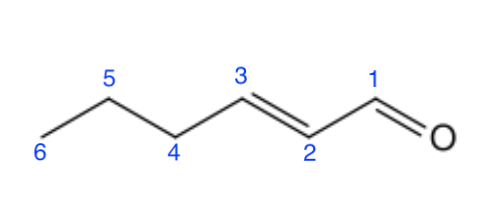
\includegraphics[width=0.7\textwidth]{navnB.png}
\end{center}
\caption{Strukturformlen for B}
\label{fig:navnB}
\end{figure}
\noindent \textbf{b.}
Det ses i \cref{fig:AmB}, at kun mersifuran og stof B indholder en carbonylgruppe.
Disse kan nemt påvises ved reaktion med 2,4-dinitrophenylhydrazin, som netop påviser carbonylgrupper.
Kun stof A vil da ikke danne gult bundfald ved reaktion med 2,4-dinitrophenylhydrazin.

For at skelne mellem mesifuran og stof B kan man så bruge Tollens reagens, der reagerer med aldehyder men ikke ketoner.
Altså vil stof B reagere med Tollens reagens, hvor mesifuran ikke vil reagere.
\begin{figure}[H]
\begin{center}
  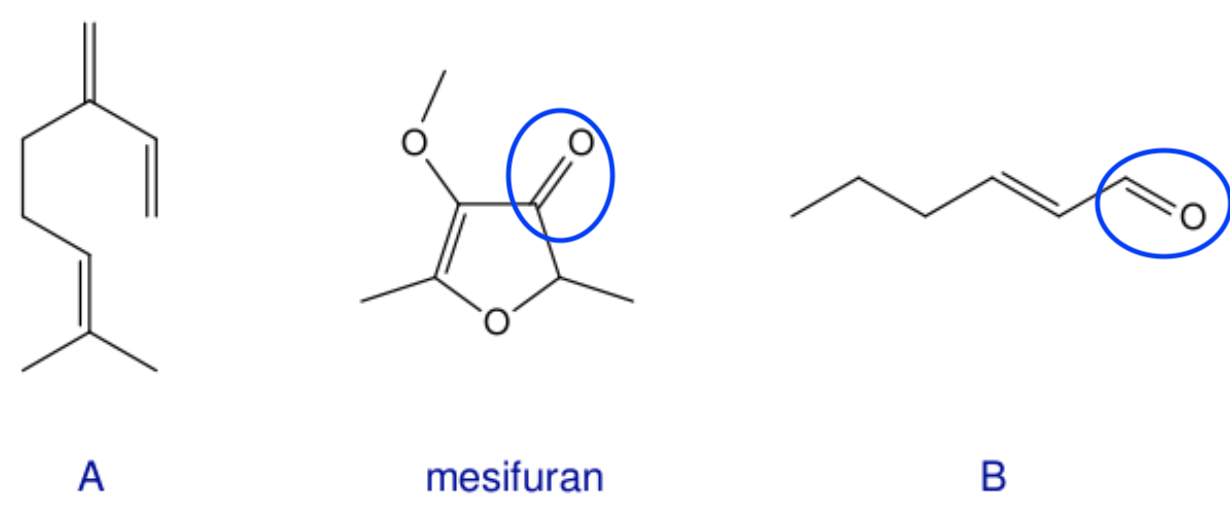
\includegraphics[width=0.7\textwidth]{AmB.png}
\end{center}
\caption{Strukturer for tre stoffer}
\label{fig:AmB}
\end{figure}
\noindent \textbf{c.}
Vi betragter \ce{^1H}-NMR-spektret for D.
Et opsummerende skema ses i \cref{tab:HNMR}.
\begin{table}[H]
\centering
\begin{tabular}{@{}lllllll@{}}
\toprule
  \makecell{Signal\\nr.} & \makecell{Kemisk skift\\(aflæst)\\$\delta$/ppm}& \makecell{Integral/areal\\(relativt antal ækvi-\\valente \ce{^1H}-atomer)}  & Opsplitning & \makecell{ Antal nabo- \\\ce{^1H}'er}  & Tilordning & \makecell{Kemisk skift\\(tabel)\\$\delta$/ppm} \\
\midrule
  1 & 0,95 & 3 & Triplet & 2 & \ce{C\textbf{H}3-CH2 -} & 0,9\\
  2 & 1,22 & 3 & Triplet & 2 & \ce{C\textbf{H}3-CH2-O-CO} & 1,2 \\
  3 & 1,62 & 2 & Sektet & 5 & \ce{CH3-C\textbf{H}2-CH2-CO-O -} & 1,7 \\
  4 & 2,30 & 2 & Triplet & 2 & \ce{-CH2-C\textbf{H}2-CO-O-C} & 2,2 \\
  5 & 4,11 & 2 & Kvartet & 3 & \ce{CH3-C\textbf{H}2-O-CO-C} & 4,1\\
\bottomrule
\end{tabular}
\caption{Tilordning af absorptionsbånd i \ce{^1H}-NMR-spektret}
\label{tab:HNMR}
\end{table}
Siden $R^1$ og $R^2$ er alkylgrupper, så må der være to \ce{CH3}-grupper i D. 
Disse må høre til signal nr. 1 og signal nr. 2.
Fra de kemiske skift og opsplitningen har vi så, at \ce{^1H}-kernerne hørende til signal nr. 2 må koble til \ce{^1H}-kernerne hørende til signal nr. 5.
Tilsvarende må \ce{^1H}-kernerne hørende til signal nr. 1 koble til \ce{^1H}-kernerne hørende til signal nr. 3, som til sidst er nødt til at koble til \ce{^1H}-kernerne hørende til signal nr. 4.

Vi har da en \ce{CH3}-gruppe bundet til en \ce{CH2}-gruppe bundet til et \ce{O}.
Derudover har vi en \ce{CH3}-gruppe bundet til en \ce{CH2}-gruppe bundet til endnu en \ce{CH2}-gruppe bundet til en \ce{CO}-gruppe.
Strukturen for D må da være som i \cref{fig:D}.
\begin{figure}[H]
\begin{center}
  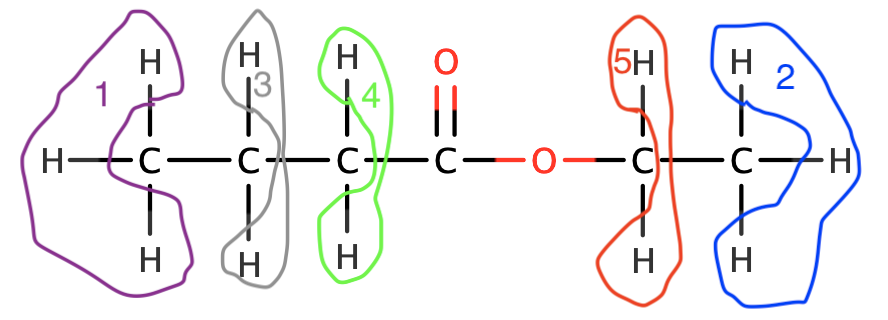
\includegraphics[width=0.7\textwidth]{D.png}
\end{center}
\caption{Struktur for D med signalerne hørende til \ce{^1H}-kernerne markeret og numereret}
\label{fig:D}
\end{figure}
\noindent \textbf{d.}
Hvis reaktionen er af første orden, så må der gælde, at 
\[
v= k \cdot c(\text{furaneol} )
\] 
Det vil sige, at punkterne på $(c(\text{furaneol} ), v)$-grafen skal ligge tilnærmelsesvist på en ret linje gennem (0,0).
Vi sætter da datapunkterne, hvor $c(\text{furaneol} ) < 5 \;\unit{\micro \textsc{m}} $ ind i Logger Pro og laver en ligefrem proportional regression, hvilket ses i \cref{fig:furanoal}.

\begin{figure}[H]
\begin{center}
  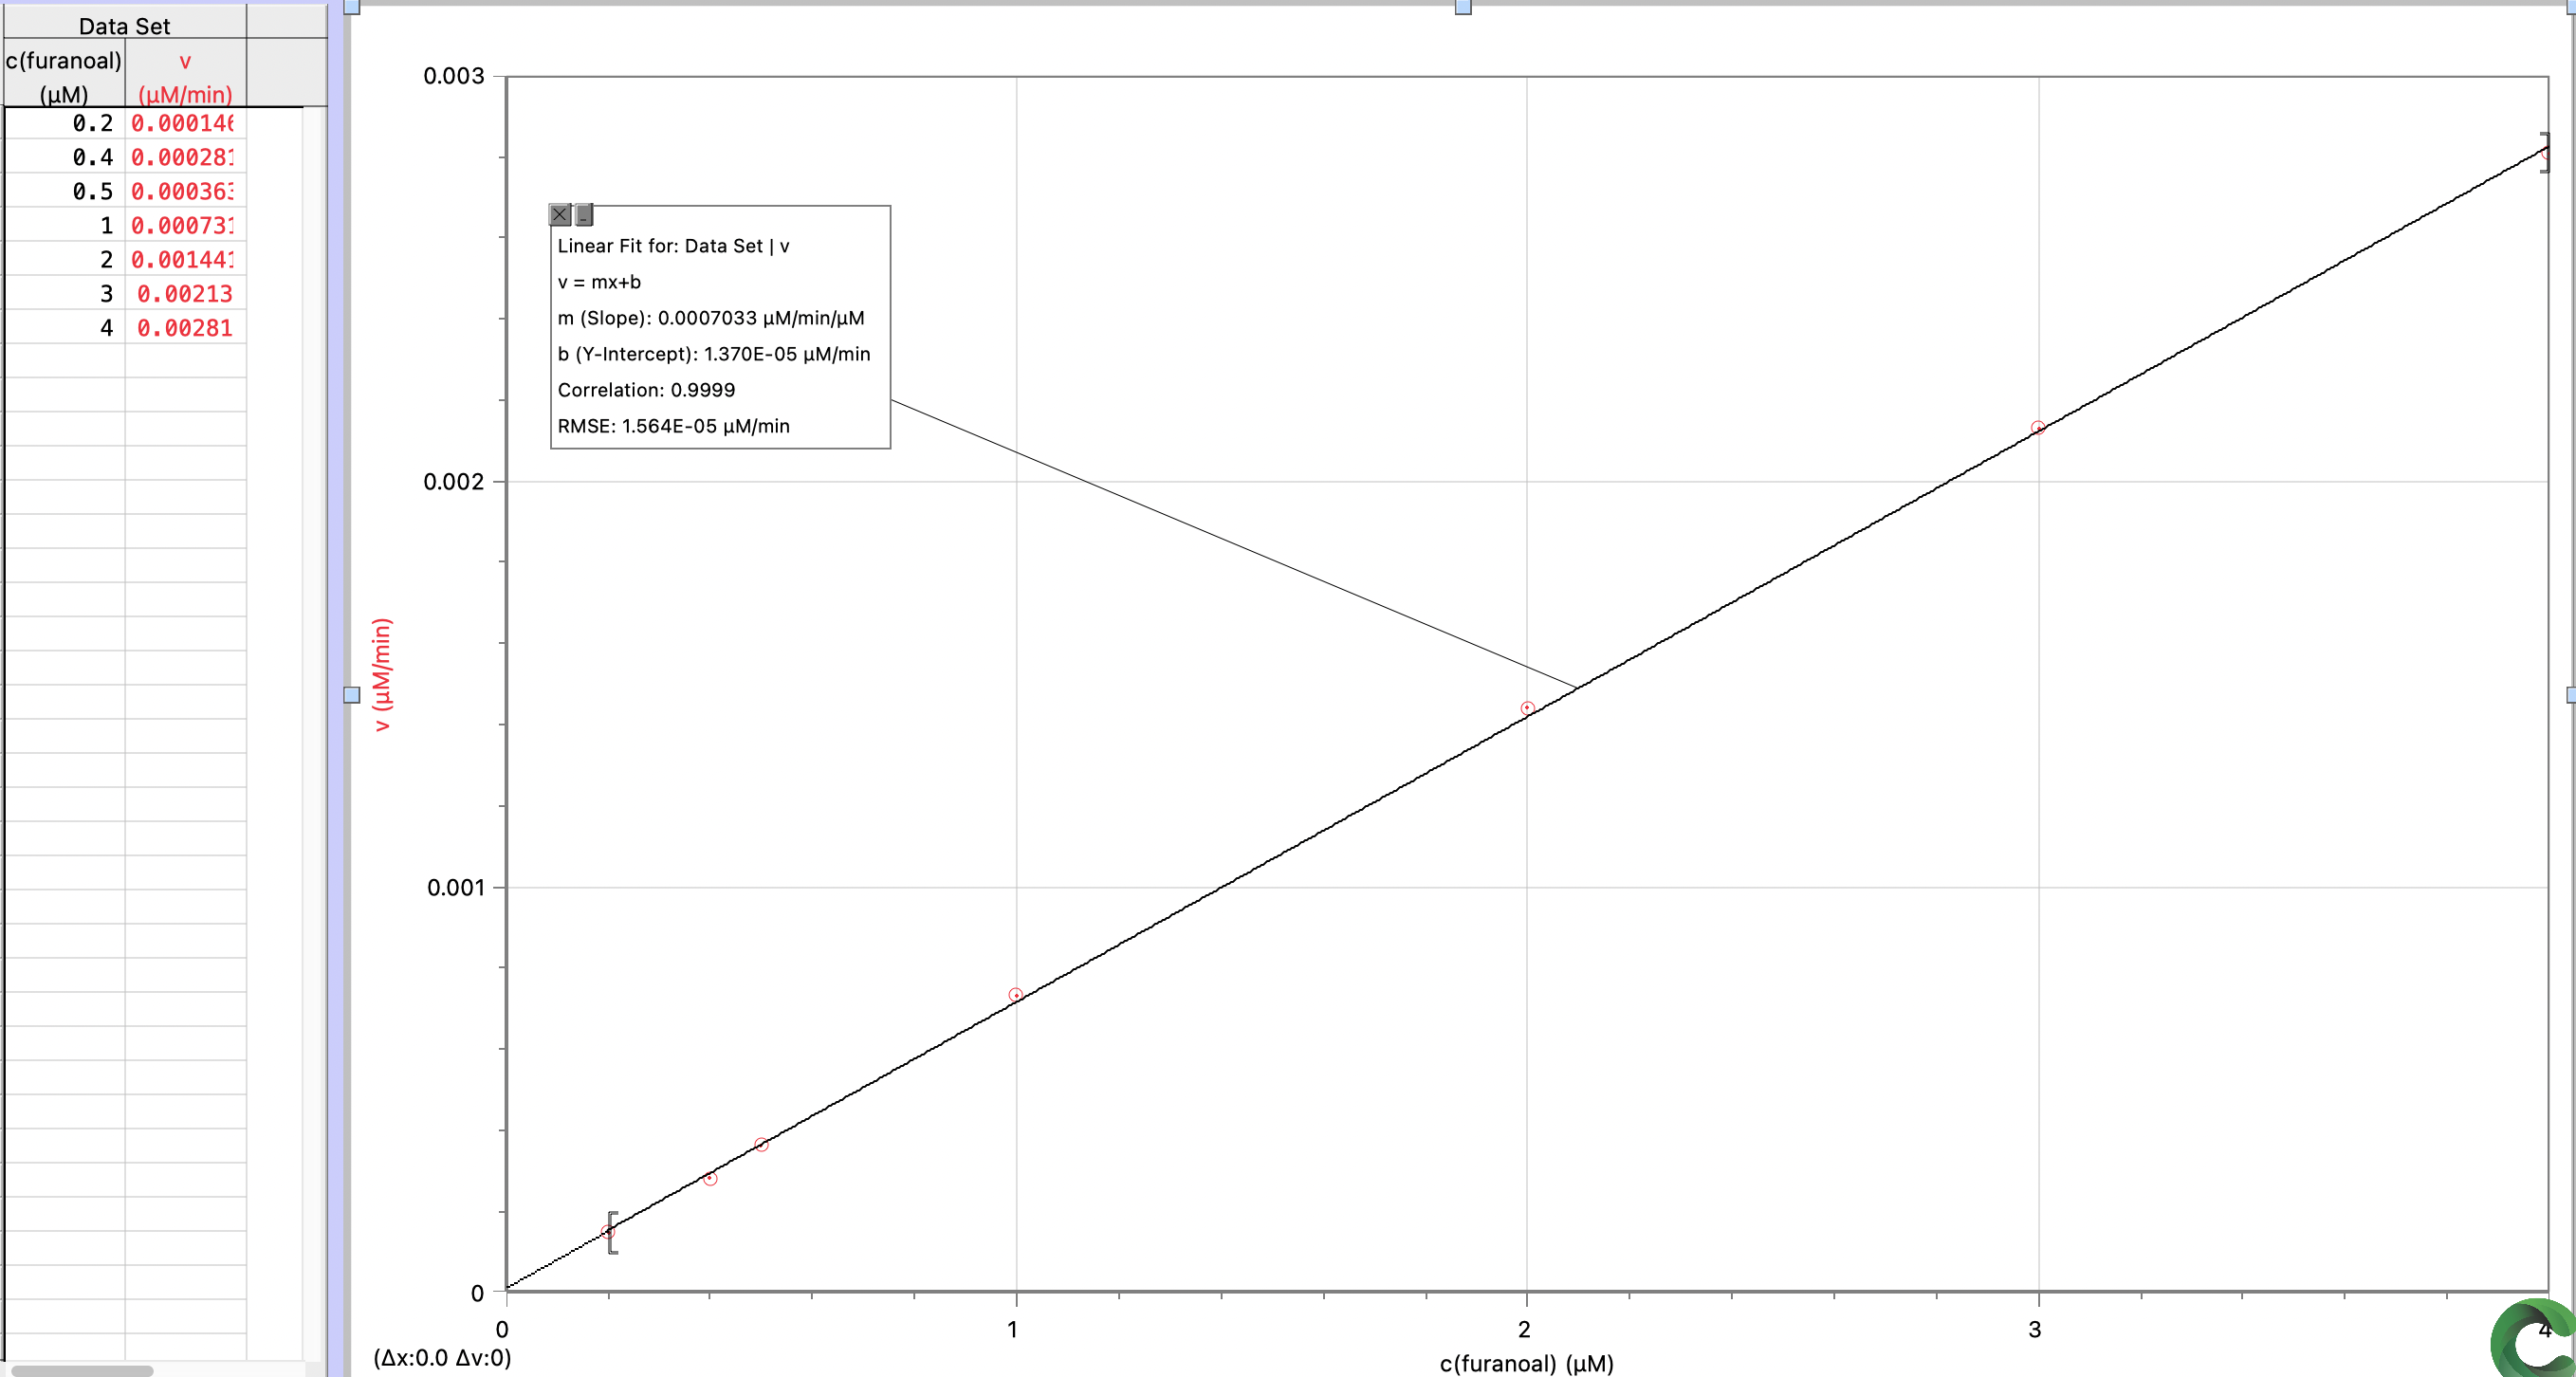
\includegraphics[width=0.7\textwidth]{furanoal.png}
\end{center}
\caption{Lineær regression på $(c(\text{furaneol} ), v)$-grafen lavet i Logger Pro}
\label{fig:furanoal}
\end{figure}
Det ses, at punkterne (hvor $c(\text{furaneol} ) < 5 \;\unit{\micro \textsc{m}} $) på $(c(\text{furaneol} ), v)$-grafen ligger tilnærmelsesvist på en ret linje gennem (0,0), og reaktionen er altså af første orden.
Fra regressionen får vi hastighedsudtrykket
\begin{equation*}
\begin{split}
  v=0,000703 \;\unit{min ^{-1}} \cdot c(\text{furaneol} ) + 1,37 \cdot 10 ^{-5} \;\unit{\micro \textsc{m}/min} 
\end{split}
\end{equation*}
Det skal bemærkes, at konstantleddet er så lille, at det kan ignoreres.

\section*{Opgave 4: Osmium - grundstoffernes sværvægter}
\sol \\
\textbf{a.}
Der er tale om en redoxreaktion, da der både sker en oxidation og en reduktion.
Dette fremgår klart af \cref{fig:redox}, hvor oxidationstallene også er angivet.
\begin{figure}[H]
\begin{center}
  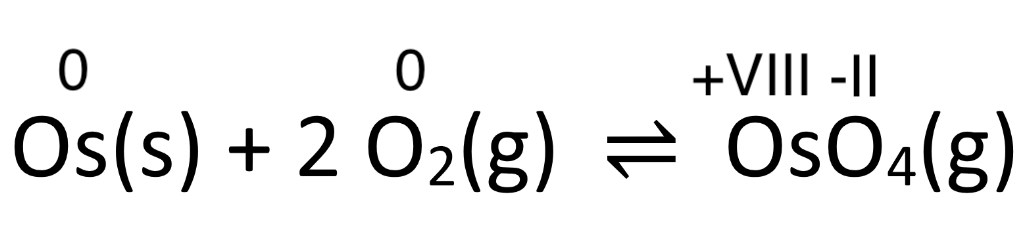
\includegraphics[width=0.7\textwidth]{redox.png}
\end{center}
\caption{Reaktionsskema med oxidationstal angivet}
\label{fig:redox}
\end{figure}
\noindent \textbf{b.}
Vi har fra figuren, at
\[
\Delta G \stst = 0,149 \;\unit{\frac{kJ}{mol \cdot K}} \cdot T -337 \;\unit{kJ/mol} 
\] 
Der gælder derudover følgende sammenhæng mellem $\Delta G \stst $ og den absolutte temperatur $T$:
\[
\Delta G \stst =-\Delta S \stst \cdot T + \Delta H \stst 
\] 
Ved at kombinere de to udtryk får vi, at 
\begin{equation*}
\begin{split}
  \Delta S \stst &= -0,149 \;\unit{\frac{kJ}{mol \cdot K}} \\
  \Delta H \stst &= -337 \;\unit{kJ/mol} 
\end{split}
\end{equation*}
Vi ser, at $\Delta S \stst < 0 $, hvilket vil sige, at ordenen øges.
Det er i overensstemmelse med reaktionsskemaet, hvor to gasmolekyler og et fast stof bliver til ét gasmolekyle.\\[1ex]
\textbf{c.}
Vi beregner først den absolutte temperatur.
\begin{equation*}
\begin{split}
T&=\frac{t \cdot \;\unit{K} }{\;\unit{\celsius} } + 273,15 \;\unit{K} \\
  &=\frac{400 \;\unit{\celsius} \cdot \;\unit{K} }{\;\unit{\celsius} }\\
  &=673,15 \;\unit{K} 
\end{split}
\end{equation*}
Vi opskriver ligevægtsloven for reaktionen for at bestemme enheden for $K$.
\[
K=\frac{p(\ce{OsO4} )}{p(\ce{O2} )^2}
\] 
Vi ser da, at enheden for $K$ må være $\;\unit{bar ^{-1}} $.

Fra van't Hoffs ligning gælder der, at
\begin{equation*}
\begin{split}
  \ln\left(K\right) = - \frac{\Delta H \stst }{R \cdot T} + \frac{\Delta S \stst }{R} \iff K=e^{- \frac{\Delta H \stst }{R \cdot T} + \frac{\Delta S \stst }{R}} 
\end{split}
\end{equation*}
Vi indsætter da de kendte værdier og beregner $K$.
\begin{equation}
\begin{split}
  K&=e^{- \frac{\Delta H \stst }{R \cdot T} + \frac{\Delta S \stst }{R}} \\
  &=e^{-\frac{-337 \cdot 10^3\;\unit{J/mol} }{8,314 \;\unit{\frac{J}{mol \cdot K} \cdot 673,15 \;\unit{K} } } + \frac{-0,149 \cdot 10^3 \;\unit{\frac{J}{mol \cdot K}} }{8,314 \;\unit{\frac{J}{mol \cdot K}} }} \\
  &\approx 2,33 \cdot 10 ^{18} 
\end{split}
  \label{eq}
\end{equation}
Ved beregningen for vi $K$ uden enhed. 
Siden vi ved enheden for $K$ er $\;\unit{bar ^{-1}} $, så må vi have 
\[
K=2,33 \cdot 10 ^{18} \;\unit{bar ^{-1}} 
\] 
Fra ligning \ref{eq} (van't Hoffs ligning) ses det, at når $T$ vokser, så aftager ligevægtskonstanten $K$ (pga. $\Delta H \stst <0$) .
Det vil sige, at ligevægten forskydes mod venstre.
Altså forskydes ligevægten mod venstre når temperaturen i reaktionsbeholderen stiger.


\end{document}
